
\tikzset{every picture/.style={line width=0.75pt}} %set default line width to 0.75pt        

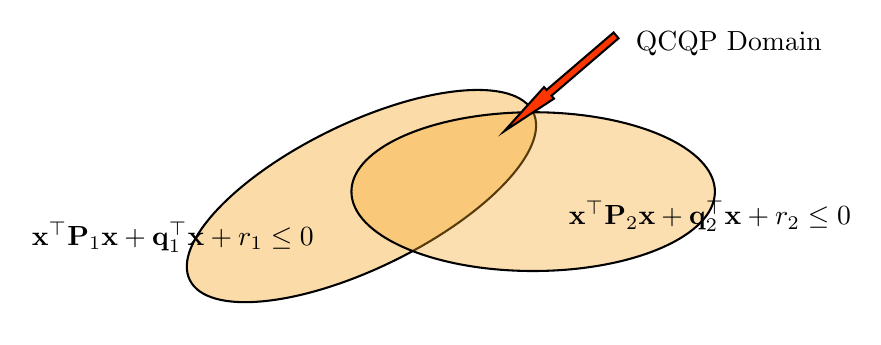
\begin{tikzpicture}[x=0.75pt,y=0.75pt,yscale=-0.75,xscale=0.75]
%uncomment if require: \path (0,300); %set diagram left start at 0, and has height of 300

%Shape: Ellipse [id:dp9898126968799086] 
\draw  [fill={rgb, 255:red, 245; green, 166; blue, 35 }  ,fill opacity=0.4 ] (103.44,199.35) .. controls (92.18,176.27) and (132.43,133.45) .. (193.35,103.71) .. controls (254.27,73.97) and (312.79,68.57) .. (324.06,91.65) .. controls (335.32,114.73) and (295.07,157.55) .. (234.15,187.29) .. controls (173.23,217.03) and (114.71,222.43) .. (103.44,199.35) -- cycle ;
%Shape: Ellipse [id:dp5973223095827915] 
\draw  [fill={rgb, 255:red, 245; green, 166; blue, 35 }  ,fill opacity=0.36 ] (207.31,142.65) .. controls (207.31,114.48) and (259.58,91.65) .. (324.06,91.65) .. controls (388.54,91.65) and (440.81,114.48) .. (440.81,142.65) .. controls (440.81,170.82) and (388.54,193.65) .. (324.06,193.65) .. controls (259.58,193.65) and (207.31,170.82) .. (207.31,142.65) -- cycle ;
%Left Arrow [id:dp11071847750004182] 
\draw  [fill={rgb, 255:red, 255; green, 53; blue, 0 }  ,fill opacity=1 ] (305.5,103.83) -- (331.05,75.5) -- (332.64,77.36) -- (375.73,40.44) -- (378.91,44.15) -- (335.82,81.07) -- (337.41,82.92) -- cycle ;

% Text Node
\draw (0,160) node [anchor=north west][inner sep=0.75pt]    {$\mathbf{x}^\top \mathbf{P}_1 \mathbf{x} + \mathbf{q}_1^\top\mathbf{x} + r_1 \leq 0$};
% Text Node
\draw (345,147) node [anchor=north west][inner sep=0.75pt]    {$\mathbf{x}^\top \mathbf{P}_2 \mathbf{x} + \mathbf{q}_2^\top\mathbf{x} + r_2 \leq 0$};
% Text Node
\draw (388,38) node [anchor=north west][inner sep=0.75pt]   [align=left] {QCQP Domain};


\end{tikzpicture}
